% !TEX root = ../main.tex

\subsection{Importance Sampling}
\label{sec:inf:foundation:importance}

Importance sampling is another common sampling method that forms the key building block
for many more advance inference schemes.  It is closely related to rejection sampling in that
it uses a proposal, i.e. $\hat{\theta}\sim q(\theta)$, but instead of going
through an accept/reject step, it assigns an \emph{importance weight} to each sample.
These importance weights act like correction factors to account for the fact that we sampled
from $q(\theta)$ rather than our target $\pi(\theta)$.

To demonstrate the key idea, consider the problem of calculating an expectation as
per~\eqref{eq:inf:expt}.  If we cannot sample exactly from $\pi(\theta)$ then we cannot
apply~\eqref{eq:inf:mc-est} directly.  However, we can rearrange the form our expectation
to generate a different \mc estimator which we can evaluate directly as follows
\begin{align}
	I:=\E_{\pi(\theta)} \left[f(\theta)\right] &=\int f(\theta) \pi(\theta) d\theta 
	= \int f(\theta) \frac{\pi(\theta)}{q(\theta)} q(\theta) d\theta \nonumber \\
	&\approx \frac{1}{N} \sum_{n=1}^{N} \frac{\pi(\hth_n)}{q(\hth_n)} f(\hat{\theta}_n)
	\quad \text{where} \quad \hat{\theta}_n \sim q(\theta) 	\label{eq:inf:importance}
\end{align}
where $\frac{\pi(\hth_n)}{q(\hth_n)} =: w_n$ is known as an importance weight.
The key trick we have applied is to multiply the integrand by $\frac{q(\theta)}{q(\theta)}$, which
equals $1$
for all points where $q(\theta) \neq 0$.  Thus if $q(\theta) \neq 0$ for all $\theta$ for which
$\pi(\theta) \neq 0$ (to avoid infinite importance weights), this has no effect on the 
expectation.  However, we can informally view the new
formulation as being the expectation of $f(\theta) \frac{\pi(\theta)}{q(\theta)}$ under the
distribution $q(\theta)$.  We can now construct a \mc estimator for this new formulation, 
by choosing $q(\theta)$ to be a distribution we can sample from.  A graphical
demonstration of importance sampling is given in Figure~\ref{fig:inf:importance} in the
more general setting where we do not have access to the $\pi(\theta)$ exactly, but only
an unnormalized version $\gamma(\theta)=\pi(\theta)Z$.  As we will show in detail in
Section~\ref{sec:inf:foundation:importance:self-norm}, we can still use importance sampling
in this case by \emph{self-normalizing} the weights.

\begin{figure}[t]
	\centering
	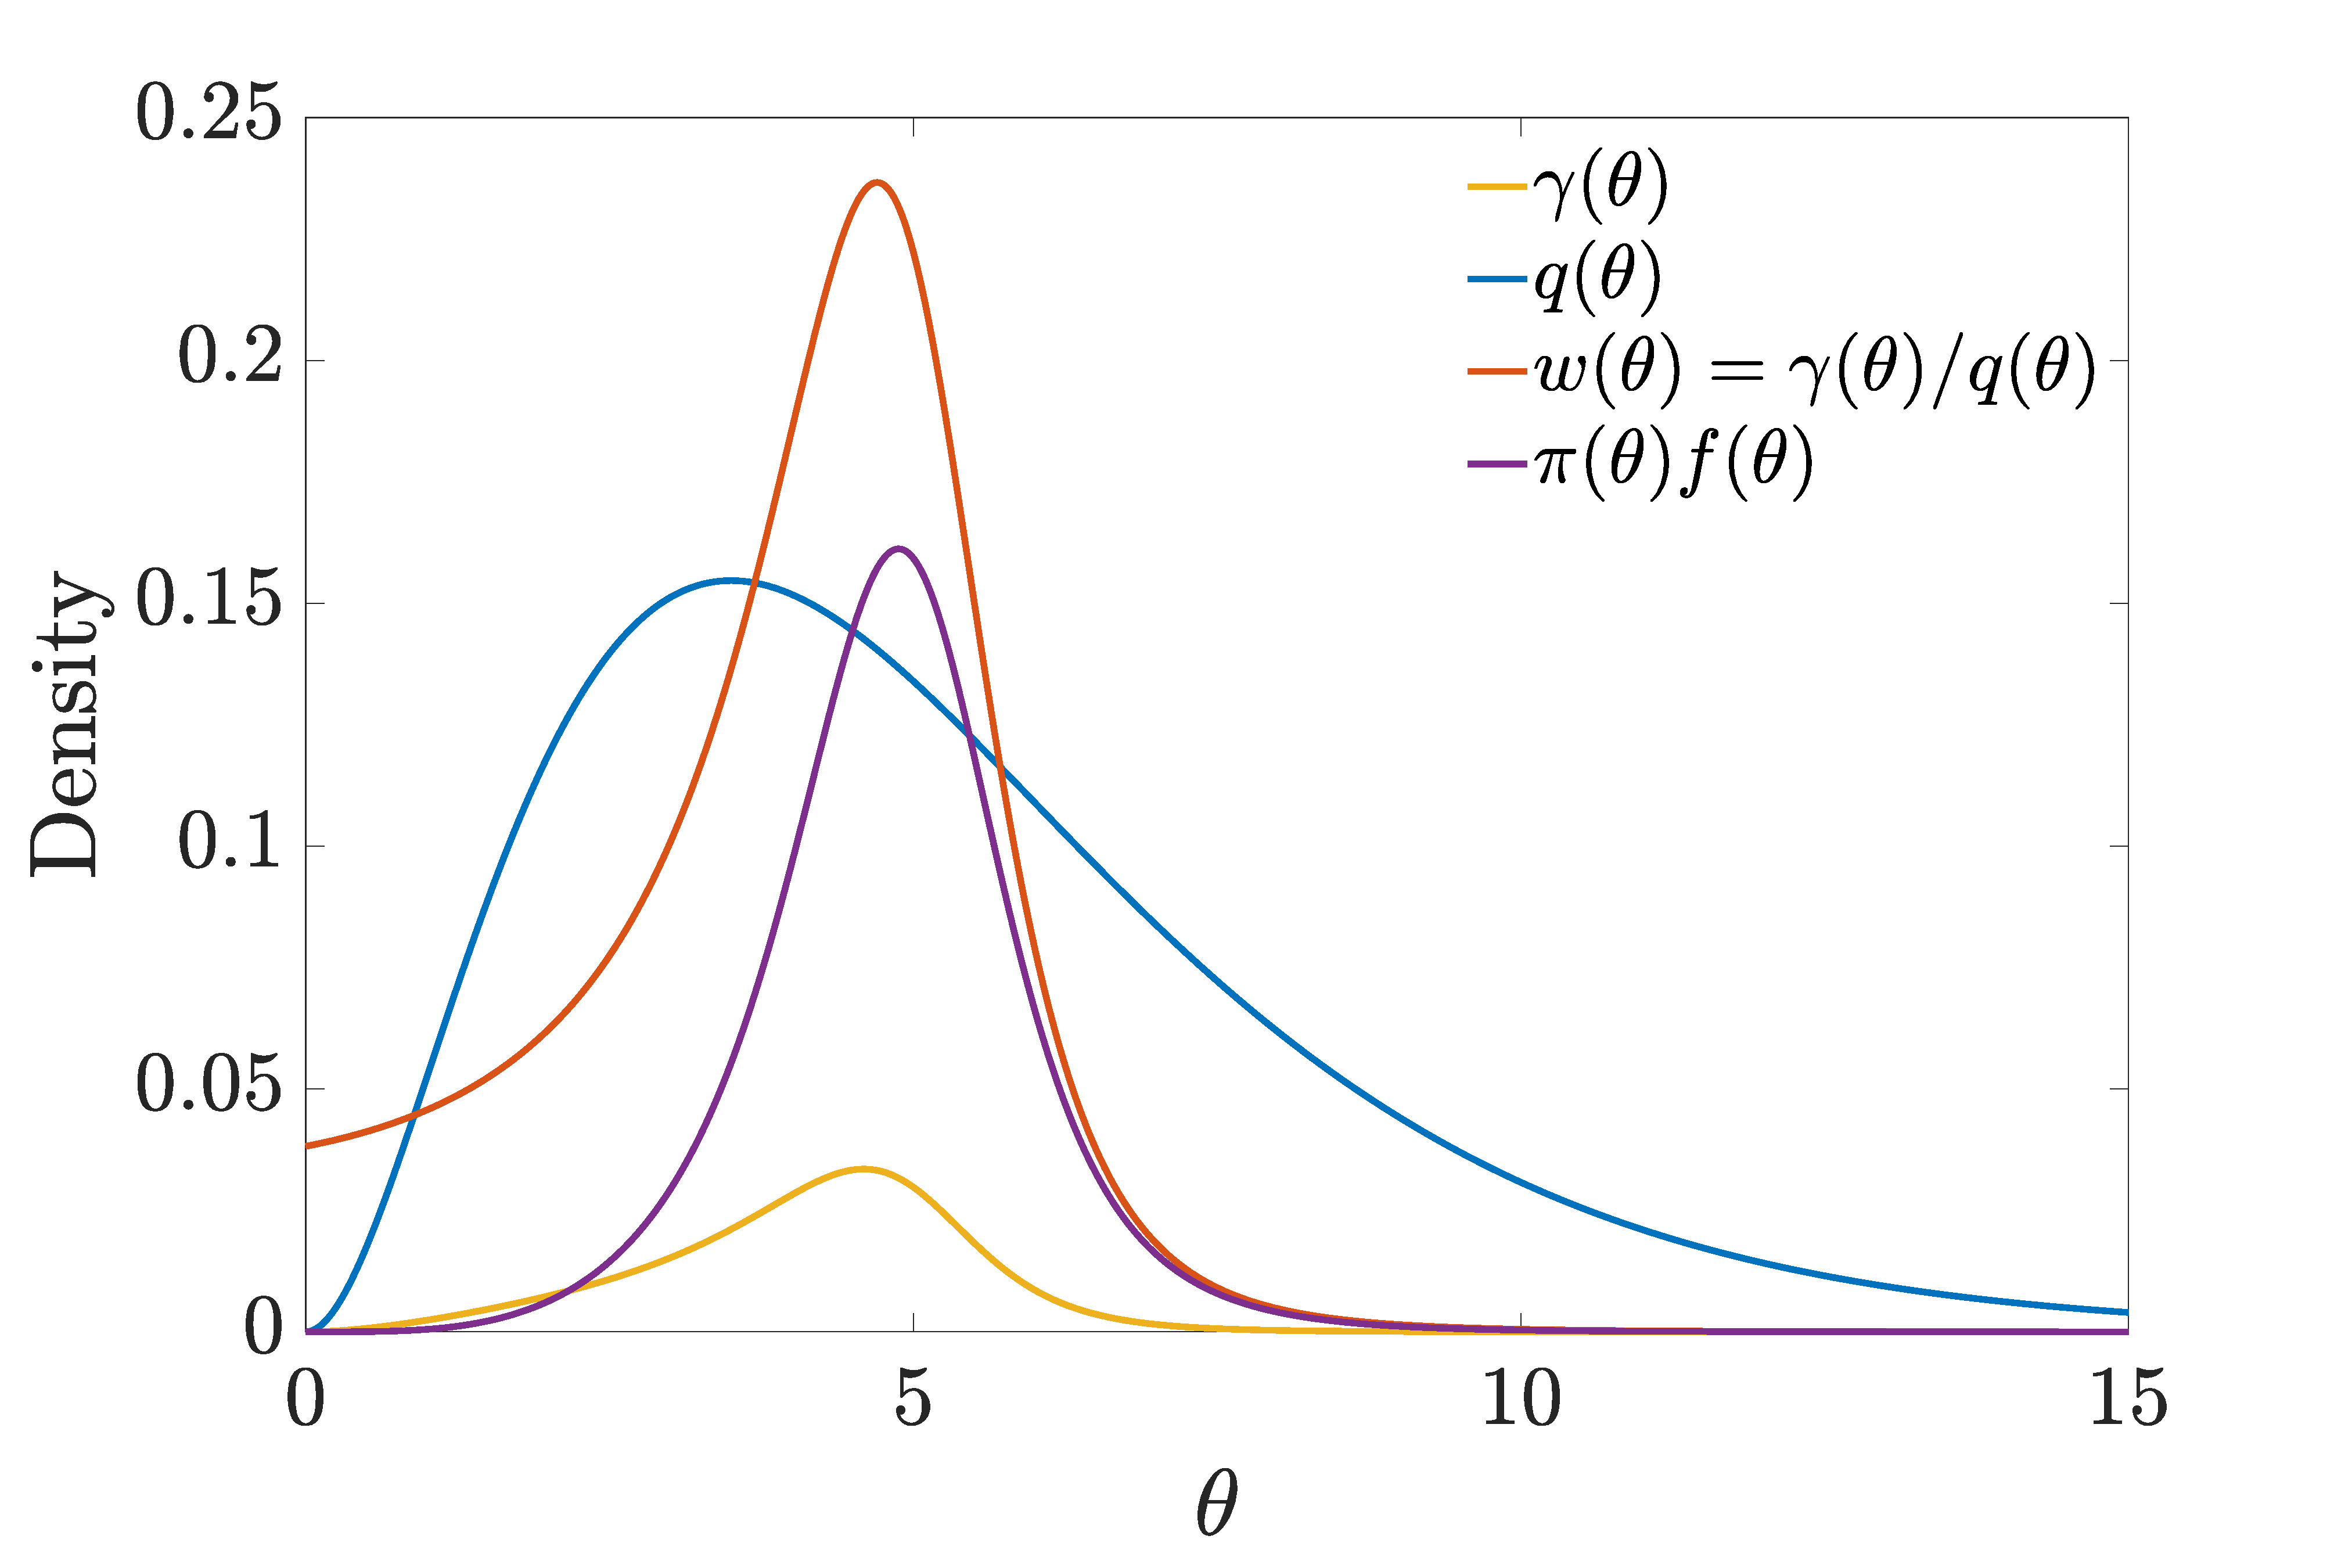
\includegraphics[width=0.5\textwidth]{importance}
	\caption{Demonstration of importance sampling for problem shown in~\eqref{eq:inf:example}.
		 We are trying to estimate $\E [\pi(\theta)f(\theta)]$: the expectation of the function $f(\theta) := \theta^2/50$
		under the posterior $\pi(\theta):=p(\theta|y=5)$ defined as per~\eqref{eq:inf:example-post}.
		We assume the setting where $\pi(\theta)$ is only known up to a normalization constant
		(see Section~\ref{sec:inf:foundation:importance:self-norm}), namely we only have access
		to $\gamma(\theta) := p(\theta)p(y=5 | \theta)$ as shown in yellow.  Our procedure is to draw
		samples independently $\hth_n \sim q(\theta)$ and then evaluate their weight 
		$w_n = w(\hth_n) = \gamma(\hth_n)/q(\hth_n)$.  This produces a set of weighted samples
		which can then be used to estimate to estimate the expectation using~\eqref{eq:inf:snis}
		(one can also use~\eqref{eq:inf:importance} if the normalized $\pi(\theta)$ is used instead of
		$\gamma(\theta)$).
		\label{fig:inf:importance}}
\end{figure}

Importance sampling has a number of desirable properties as an inference method.
In particular, it is both unbiased and consistent.  The former can be shown trivially
as follows
\begin{align}
\E \left[\frac{1}{N} \sum_{n=1}^{N} \frac{\pi(\hth_n)}{q(\hth_n)} f(\hat{\theta}_n)\right] &=
\frac{1}{N} \sum_{n=1}^{N} \E _{q(\theta_n)}\left[\frac{\pi(\hth_n)}{q(\hth_n)} f(\hat{\theta}_n)\right] \nonumber \\
&=\E _{q(\theta_1)}\left[\frac{\pi(\hth_1)}{q(\hth_1)} f(\hat{\theta}_n)\right] =
\E _{\pi(\theta)}\left[f(\theta)\right]
\end{align}
where we have effectively stepped backwards through~\eqref{eq:inf:importance}.\footnote{Note that
	this unbiasedness result does not pass over to the self-normalized variant given 
	in Section~\ref{sec:inf:foundation:importance:self-norm}.}
Given this unbiasedness result, $L^2$ convergence, and thus convergence in probability,
can be shown in the same manner as~\eqref{eq:inf:LLN-informal} by replacing
each $f(\hth_n)$ with $\frac{\pi(\hth_n)}{q(\hth_n)} f(\hat{\theta}_n)$, leading to the
same result except that $\sigma_{\theta}$ is now
\begin{align}
\label{eq:inf:sigma-imp}
\sigma_{\theta}^2 = \E_{q(\theta)} \left[\left(\frac{\pi(\hth_n)}{q(\hth_n)} f(\hat{\theta}_n)-I\right)^2\right]
= \var_{q(\theta)} \left[\frac{\pi(\theta)}{q(\theta)} f(\theta)\right].
\end{align}
Almost sure convergence of importance sampling can be similarly shown using
the strong law of large numbers.

The form of~\eqref{eq:inf:sigma-imp} provides substantial insight into how
best to set the proposal: we have shown that the mean squared error of an
importance sampler is directly proportional to $\var \left[f(\theta)\pi(\theta)/q(\theta)\right]$,
thus the lower this term is, the better the expected performance of our
estimator.  One obvious question is what is the optimal proposal $q^*(\theta)$?
It turns out that $q^*(\theta) = \frac{\pi(\theta)\left|f(\theta)\right|}
{\int \pi(\theta)\left|f(\theta)\right|d\theta}$
\citep{kahn1953methods,owen2013mc}, which can be
 shown as follows where we will make use of Jensen's inequality
\begin{align}
\var_{q^*(\theta)} &\left[\frac{\pi(\theta)}{q^*(\theta)} f(\theta)\right] =
\E_{q^*(\theta)} \left[\left(\frac{\pi(\theta)}{q^*(\theta)} f(\theta)\right)^2\right]
-\left(\E_{q^*(\theta)} \left[\frac{\pi(\theta)}{q^*(\theta)} f(\theta)\right]\right)^2
\nonumber \\
 &= \int \frac{\pi(\theta)^2 f(\theta)^2}{q^*(\theta)} d\theta
 -I^2 
 = \left(\int \pi(\theta) \left|f(\theta)\right| d\theta\right)^2
 -I^2 \label{eq:inf:opt-q-line2}\\
 &\le \int \left(\frac{\pi(\theta) f(\theta)}{q(\theta)}\right)^2 q(\theta) d\theta
 -I^2 =\var_{q(\theta)} \left[\frac{\pi(\theta)}{q(\theta)} f(\theta)\right] \label{eq:inf:opt-q}.
\end{align}
Here we have shown that the variance for $q^*(\theta)$ is less than or equal to the variance
using an arbitrary $q(\theta)$.  It must therefore be the optimal proposal.
A further point of note is that if $f(\theta)\ge0 \; \forall \theta$ (or 
$f(\theta)\le0 \; \forall \theta$), 
then~\eqref{eq:inf:opt-q-line2} will equal zero giving a zero variance estimator:
each importance weight will be equal to the  $I/f(\theta)$ and thus $I$
can be calculated by evaluating a single point.  

Though it will typically be impossible to find $q^*(\theta)$ in practice, it still 
provides a guide as to what constitutes a good proposal -- we want
$\pi(\theta)\left|f(\theta)\right|/q(\theta)$ to be as close to constant as possible.
In particular, we need to be careful to avoid scenarios where 
$\frac{\pi(\theta)\left|f(\theta)\right|}{\int \pi(\theta)\left|f(\theta)\right|d\theta}
\gg q(\theta)$ as this will cause the ratio to explode, leading to high variances.
A consequence of this is that we want $q(\theta)$ to have \emph{light tails}
compared to $\pi(\theta)\left|f(\theta)\right|$ to ensure that the ratio does not
systematically increase as $\theta$ moves away from the modes of $q(\theta)$.
Aside from the clear practical issues, If this requirement does not hold, then
it can easily be the case that $\sigma_{\theta}=\infty$ and thus that the estimator
has infinite variance.  Consider, for example, the case where 
$\pi(\theta) = \mathcal{N}(\theta ; 0,1)$, $f(\theta)=\theta$, and
$q(\theta) = \mathcal{N}(\theta ; 0,s^2)$ (Example 9.1 from~\cite{owen2013mc}).
Noting that the mean, $I$, is zero by symmetry and defining $\nu = \frac{1}{2s^2}-1$, we have that
%, $\mathrm{erf}$ is the error function for which $\mathrm{erf}(\infty)=-\mathrm{erf}(-\infty)=1$)
\begin{align}
\sigma_{\theta}^2 &= \int_{-\infty}^{\infty} \theta^2 \frac{\left(\exp\left(-\theta^2/2\right)/\sqrt{2\pi}\right)^2}
{\exp\left(-\theta^2/\left(2s^2\right)\right)/\sqrt{2\pi s^2}} d\theta
-I^2 \nonumber = \frac{s}{\sqrt{2\pi}}  \int_{-\infty}^{\infty} \theta^2 \exp \left(\theta^2 \nu\right) d\theta.
%&= \frac{s}{\sqrt{2\pi}}  \int_{-\infty}^{\infty} \theta^2 \exp \left(-\frac{\theta^2}{2}\left(2-\frac{1}{s^2}\right)\right) d\theta
%&= \frac{s}{\sqrt{2\pi}}  \left[
%\frac{\sqrt{\frac{\pi}{2}} \mathrm{erf} \left(\frac{\theta}{\sqrt{2}} \sqrt{2-\frac{1}{s^2}}\right)}
%{\left(2-\frac{1}{s^2}\right)^{3/2}}-\frac{\theta \exp \left(-\frac{\theta^2}{2}\left(2-\frac{1}{s^2}\right)\right) }{\left(2-\frac{1}{s^2}\right)}
%\right]_{\theta=-\infty}^{\theta=\infty} \nonumber \\
%&= \frac{s}{\left(2-\frac{1}{s^2}\right)^{3/2}}
\end{align}
Now this integral is clearly only finite for $\nu < 0$ (as otherwise the integrand
is $+\infty$ and $\theta = \pm \infty$ and finite elsewhere).  Therefore, $\sigma_{\theta}$
is only finite when $s^2>1/2$.  In other words, we only get a finite estimator
in this case if the proposal variance is at least half that of the target distribution $\pi(\theta)$!
The highlights the pitfalls of having insufficiently heavy tails on our proposal.
Overcoming these will typically require careful setup of the proposal on a case-by-case basis,
for example, choosing a distribution type for the proposal that is known to have heavier tails 
than $\pi(\theta)$.

\subsubsection{Self-Normalized Importance Sampling}
\label{sec:inf:foundation:importance:self-norm}

In the previous section we presumed that we have access to a normalize version of the target
$\pi(\theta)$.  Typically this will not be the case and we will only have access to an
unnormalized target $\gamma(\theta)=\pi(\theta)Z$ as per~\eqref{eq:inf:unnorm-target},
for example only having access to the joint rather than the posterior in the Bayesian inference setting.
In a less common, but still plausible situation, it may also only be possible to evaluate the proposal
up to a normalization constant.
We now show how one can still use importance sampling in these scenarios, by
\emph{self-normalizing} the importance weights.

The key idea for self-normalized importance sampling (SNIS) is that the weights provide
an unbiased and consistent estimator of the marginal likelihood
\begin{align}
Z_N &= \frac{1}{N} \sum_{n=1}^{N} w_n, \\
\E [Z_N] &= \frac{1}{N} \sum_{n=1}^{N} \E[w_n] =\E_{q(\hth_1)}[\gamma(\hth_1)/q(\hth_1)] = Z.
\end{align}
Now as $\E_{q(\theta)}\left[\frac{\gamma(\theta)}{q(\theta)}f(\theta)\right]=
E_{q(\theta)}\left[\frac{\pi(\theta)}{q(\theta)} Zf(\theta)\right]=Z\;\E_{\pi(\theta)} \left[f(\theta)\right]$, we can 
use our samples to construct \mc estimators for both $Z$ and $Z\;\E_{\pi(\theta)} \left[f(\theta)\right]$ and use the ratio
of our estimates to get an estimate for $E_{\pi(\theta)} \left[f(\theta)\right]$
\begin{align}
\label{eq:inf:snis}
\E_{\pi(\theta)} \left[f(\theta)\right] \approx \frac{\sum_{n=1}^{N} w_n f(\hth_n)}{\sum_{n=1}^{N} w_n}
\quad \mathrm{where} \quad \hth_n \sim q(\theta), \quad w_n = \frac{\gamma(\hth_n)}{q(\hth_n)}.
\end{align} 
This can alternatively be expressed as
$\E_{\pi(\theta)} \left[f(\theta)\right] \approx \sum_{n=1}^{N} \bar{w}_n f(\hth_n)$
where $\bar{w}_n = \frac{w_n}{\sum_{n} w_n}$ are the normalized importance 
weights such that $\sum_{n=1}^N\bar{w}_n = 1$.  

The consistency of~\eqref{eq:inf:snis} follows by Slutsky's
 from the individual consistency of both the numerator and the denominator to 
$Z\;\E_{\pi(\theta)} \left[f(\theta)\right]$ and $Z$ respectively.
However, unlike~\eqref{eq:inf:importance},~\eqref{eq:inf:snis} is a \emph{biased} estimator
for finite $N$.  This is
because the numerator and denominator are correlated and because 
even though $Z_N$ is an unbiased estimator of $Z$, $1/Z_N$ is not an unbiased
estimator of $1/Z$. The latter follows directly from Jensen's inequality
noting that inversion is a convex function for strictly positive inputs,
\begin{align}
\E \left[\frac{1}{\sum_{n=1}^{N} w_n}\right] \ge \frac{1}{\E \left[\sum_{n=1}^{N} w_n\right]} = \frac{1}{Z},
\end{align}
where equality holds if and only if $Z_N$ is a zero variance estimator for $Z$ (which
typically happens only in the limit $N\rightarrow\infty$).  However, it can be shown that the
bias decreases at a rate $O(1/N)$ (see e.g.~\cite{doucet2009tutorial}), whereas the
standard deviation of the estimate decreases at a rate $O(1/\sqrt{N})$.  Thus the bias
becomes dominated as $N\rightarrow\infty$.

Strangely, even when the normalization constant
is known, the self-normalized importance sampler can still be lower variance~\citep{owen2013mc}.
Therefore, with the bias becoming dominated, it can actually be preferable to use
SNIS even when the normalized target is known.  Note also that the optimal proposal in
the SNIS case varies slightly from the $q^*(\theta)$ derived earlier in the Section
and is instead~\citep{hesterberg1988advances}
\begin{align}
q^*_{\mathrm{SNIS}} (\theta) = \frac{\pi(\theta)\left|f(\theta)-I\right|}
{\int \pi(\theta)\left|f(\theta)-I\right|d\theta}.
\end{align}
As a consequence, there is a minimum variance on the SNIS estimator, unlike in the
pre-normalized case where $q^*(\theta)$ was a zero variance estimator  was possible
if $f(\theta)\ge0 \; \forall \theta$.

\subsubsection{Unknown $f$}
\label{sec:inf:foundation:importance:unk-f}

So far we have assumed that we are using importance sampling to calculate an expectation 
of a known function.  In practice, there will be many scenarios, particularly in the Bayesian inference setting,
where $f(\theta)$ is not known ahead of time and we instead desire to generate samples
for some future unknown use.  For example, in Section~\ref{sec:part:smc} we will introduce the concept
of \emph{sequential Monte Carlo} where we will typically have multiple importance sampling steps
before any target function is itself evaluated.
When no $f(\theta)$ is specified, we can carry out importance sampling in the
same fashion, sampling from $q (\theta)$ and returning a set of \emph{weighted} samples
$\{\hth_n,w_n\}_{n=1:N}$ where the weights are equal to $\gamma(\hth_n) / q(\hth_n)$ as before.
Here we can think of importance sampling as approximating the posterior with a series of deltas
functions, namely
\begin{align}
\label{eq:inf:imp-post-est}
\pi (\theta) \approx \hat{\pi}(\theta) := \sum_{n=1}^{N} \bar{w}_n \delta_{\hth_n} (\theta)
\end{align}
where $\delta_{\hth_n} (\theta)$ are delta functions centred at $\hth_n$.

Importance weights are multiplicative when doing conditional
sampling: if we sample $\hth_n \sim q_1(\theta)$ then $\hat{\phi}_n | \hth_n \sim q_2(\phi | \hth_n)$
when targeting $\gamma_1(\theta)\gamma_2(\phi|\theta)$ then the importance weight is 
\begin{align}
\label{eq:inf:prod-imp-weights}
\frac{\gamma_1(\hth_n)\gamma_2(\hat{\phi}_n|\hth_n)}{q_1(\hth_n)q_2(\hat{\phi}_n | \hth_n)}
=\frac{\gamma_1(\hth_n)}{q_1(\hth_n)}
\times\frac{\gamma_2(\hat{\phi}_n|\hth_n)} {q_2(\hat{\phi}_n | \hth_n)}= w_{n,1} \times w_{n,2}.
\end{align}
This is known as sequential importance sampling and means that we can propagate importance
weighted samples through a computational system and retain a valid importance
sampler with the standard properties such as unbiasedness (presuming the weights are not self-normalized) 
and consistency.

Again a natural question in this ``unknown $f$'' setting is what is the optimal proposal $q^*(\theta)$?
This is a somewhat more challenging and subjective question than when $f$ is known as the
optimality will depend on what the samples are eventually used for.  In particular, even if we do
not known $f$ precisely, it may be the case that we believe some $f$ are more likely than others, or we
may know that $f$ lives within some space of possible functions, for example functions that have
a countable number of discontinuities.  

One simple, but insightful approach, is to consider the 
\emph{minimax} optimal proposal, i.e. the proposal that has the minimum error if $f$ is the
most adversarial possible function for that proposal.
Imagine that we have $N$ weighted samples
$\{\hth_n,w_n\}_{n=1:N}$, with $N$ corresponding evaluations $f_n := f(\hth_n)$.
We use these to calculate an estimate $I_N$ for the target $I$.
Now assume that each $w_n\ge0$, $\sum_{n=1}^{N}w_n = 1$, and $\sum_{n=1}^{N} |f_n-I| = N$ to
preclude the ability to provide an improved solution simply by scaling the problem.
The error for the estimator is given by
\begin{align}
\left|I_N-I\right| = \left|\sum_{n=1}^{N} w_n f_n - I\right| = \left|\sum_{n=1}^{N} w_n (f_n - I)\right|.
\end{align}
For any given set of weights, the most adversarial set of function evaluations is
to have all our error at the largest weight, i.e. $|f_{n^*}-I| = N$ and $|f_{n}-I| = 0, \; n\neq n^*$
where $n^*$ is the index of the largest weight.  For this set of adversarial $f_n$, the
lowest error is achieved when each of the weights are equal.  Consequently,
we see that the minimax proposal under our assumptions is $q(\theta)=\pi(\theta)$.
This result is perhaps not surprising as it effectively states that the best sample representation 
of $\pi(\theta)$ for an unknown future use is to sample from that distribution directly.
As shown in the next section, this proposal will also minimize the variance of the estimator
under the assumption that the $f_n$ are independent.

Nonetheless, this point of view is not without criticism in the 
literature~\citep{o1987monte,ghahramani2003bayesian,briol2015probabilistic}.  Most of 
this criticism revolves around the valid point that in practice the value of $f(\theta)$ 
does convey information about $f(\theta+\varepsilon)$ and so the correlation between 
samples such be taken into account when making an estimation.  Though the thrust of
this argument is mostly directed towards changing the Monte Carlo method, and in particular
importance sampling, at a more fundamental level, the same arguments would still suggest
that it can be beneficial to use a proposal that is more diffuse than the target, thereby
reducing the correlation between the produced samples.

\subsubsection{Effective Sample Size}
\label{sec:inf:foundation:ess}

In this section we consider an important diagnostic for the performance of importance
sampling based schemes, the \emph{effective sample size} (ESS).  In
Section~\ref{sec:inf:mc:clt} we showed how an uncertainty estimate for a \mc
estimator can be derived.  However, this cannot be used when $f$ is unknown
and even if $f$ is known, it does necessarily convey much information about how effective
our proposal is compared to how effective it \emph{could} be.  The ESS instead informally provides an
estimated measure of the amount of information stored in our weighted sample set.
The more information stored in the samples, the better our approximation of the posterior, and,
at a high level, the more evenly balanced our weights, the more information they encode.
Therefore, the ESS is a measure of how many unweighted samples would be required to
convey the same information about the posterior as the weighted sample set.

The weighted average of $N_e$ independent evaluations $\{f_n\}_{n=1}^N$, each 
with individual variance $\sigma^2$,
has variance $\sigma^2 / N_e$ as we showed in~\eqref{eq:inf:LLN-informal}.  Therefore,
we can calculate the ESS of a set of weighted samples by comparing the variance of our 
weighted estimated to the variance of an estimate using a
set of unweighted evaluations. More specifically, the ESS will be the number of unweighted evaluations
$N_e$ that gives an equivalent variance to our weighted estimate as follows where we
will make use of the assumption that the $f_n$ are independent
\begin{align}
\frac{\sigma^2}{N_e} &= \var \left[\frac{\sum_{n=1}^{N} w_n f_n}{\sum_{n=1}^{N} w_n} \middle| 
														\{w_n\}_{n=1}^N\right] = \sum_{n=1}^{N} \left(\frac{\sum_{n=1}^{N} w_n}{\sum_{n=1}^{N} w_n} \right)^2 \var [f_n] 
														= \frac{\sigma^2\sum_{n=1}^{N} w_n^2}{\left(\sum_{n=1}^{N} w_n\right)^2}.
\end{align}
Now rearranging for $N_e$ we get
\begin{align}
\label{eq:inf:ess}
N_e = \frac{\left(\sum_{n=1}^{N} w_n\right)^2}{\sum_{n=1}^{N} w_n^2} = \frac{1}{\sum_{n=1}^{N} \bar{w}_n^2}
\end{align}
which completes our definition for the effective sample size.\footnote{Note that it is sometimes necessary
	to collapse identical weighted samples to a single sample when
	calculating~\eqref{eq:inf:ess}, such as when doing doing resampling (see Section~\ref{sec:inf:foundation:resampling})
	}
It transpires that $N_e$ is
independent of $f$, so we can still use the ESS as a diagnostic when $f$ is unknown.
It is straightforward to show using Jensen's inequality we have that $N_e\le N$ with equality
holding if and only if all the weights are equal.  On the other hand, if all but one of the weights
is zero, then $N_e=1$.  These two extremes respectively occur when the proposal
is equal to the target, $q(\theta)=\pi(\theta)$, and when the proposal provides a very poor
representation of the target.  The ESS is often therefore used for \emph{proposal adaptation},
as a larger value of the ESS generally indicates a better proposal.

However, the ESS is far from a perfect measure of sample quality.  For example, if the proposal
perfectly matches one of the modes of the target but completely misses another larger mode, the
ESS will usually be very high, even though the samples provide a very poor representation of the
target.  It is not uncommon in practice to see the ESS drop drastically as more samples are added,
due to the addition of a new dominating sample, typically indicating a region of significant target probability
mass that had previously been missed.  Nonetheless, the ESS is still a very useful performance
metric and is usually a reliable indicator for whether our importance sampling is struggling.  
In particular, though the possibility of missing modes means that although it is possible for the ESS to be 
high even when the approximation of the posterior is poor, if the ESS is low then the approximation 
of the posterior will always be poor and any subsequent estimates will, in general, be high variance.

\subsubsection{Resampling}
\label{sec:inf:foundation:resampling}

A useful feature of SNIS is that it can be used to produce unweighted samples
by \emph{sampling with replacement} from the set of produced samples in proportion
to the sample weights.  This procedure is typically known as resampling, because we
are resampling samples from the empirical distribution of our original samples.
It allows us to generate unweighted samples with importance sampling which are
approximately distributed according to $\pi(\theta)$, with this approximation becoming
exact in the limit $N\rightarrow\infty$.  
Resampling on its own always lead to a higher variance estimator than using~\eqref{eq:inf:snis}
directly.   However, in addition to  being necessary when unweighted samples are required,
it will be a key component in the so-called particle-based inference methods discussed
in Chapter~\ref{chp:part}.  
%For example, when interleaved with sequential importance sampling,
%this leads to the sequential importance resampling algorithm which is the backbone of 
%sequential \mc methods.

Mathematically, we can express resampling as producing a set unweighted resampled
samples $\left\{\tilde{\theta}_n\right\}_{n=1}^N$ using
\begin{align}
\label{eq:inf:resampling}
\tilde{\theta}_n = \hth_{a_n} \quad \mathrm{where} \quad
a_n \sim \textsc{Discrete}\left(\left\{\bar{w}_n\right\}_{n=1}^N\right).
\end{align}
Here $\left\{a_n\right\}_{n=1}^N$ are known as ancestor indices as they indicate which ancestor
in the original sample set each unweighted sample originated from.  Note that the $a_n$ need
not be drawn independently and typically are not;~\eqref{eq:inf:resampling} instead conveys
the required marginal distribution for each $a_n$.  

Considering the approximation of the
posterior provided by importance sampling given in~\eqref{eq:inf:imp-post-est}, we can view
resampling as producing the approximation
\begin{align}
\label{eq:inf:resampling-post}
\tilde{\pi}(\theta) := \sum_{n=1}^{N} \frac{k_n}{N} \delta_{\hth_n} (\theta)
\end{align}
where $k_n$ is the number times the sample $\hth_n$ appears in the resampled sample
set $\left\{\tilde{\theta}_n\right\}_{n=1}^N$.  Provided that $\E[k_n | \{w_n\}_{n=1}^N] = Nk_n$,
then it directly follows that $\tilde{\pi}(\theta)$ is an unbiased estimator for $\hat{\pi}(\theta)$.
Consequently the $L^2$ convergence, and thus consistency, of SNIS with resampling follows
directly from the $L^2$ convergence of SNIS.
	
There are a number of different methods one can use for resampling~\citep{douc2005comparison}.  They all share in 
common the requirements above, but vary in correlations between the $a_n$.  The simplest
method, \emph{multinomial resampling}, simply involves sampling each $a_n$ independently,
such that the $k_n$ have a multinomial distribution.  Though simple, this method is generally
inadvisable as it adds unnecessary variation to the resampling compared to methods using randomized
quasi-Monte Carlo~\citep{l2005recent}, such as systematic 
resampling~\citep{carpenter1999improved,whitley1994genetic},\footnote{Note that systematic resampling as it is now known is
	somewhat confusingly referred to as stratified resampling in the former of these papers and universal
	sampling in the latter.}
or other variance reduction techniques, such as stratified 
resampling~\citep{kitagawa1996monte} and residual resampling~\citep{whitley1994genetic}.
Though residual resampling is a little more complicated (see~\cite{douc2005comparison}),
stratified and systematic resampling can be viewed as small changes on the underlying random
number draws made in multinomial resampling.  The typical way to drawn from a multinomial
distribution with $N$ trials and probabilities $p_1,\dots,p_K$ is to make $N$ independent
draws from a unit uniform distribution, $u_n \iid \textsc{Uniform}(0,1) \; \forall n\in1,\dots,N$
and then to bin these into the intervals between the cumulative probabilities
$P_0 = 0, \; P_{j} = \sum_{\ell=1}^{j} p_{\ell}, \; \forall j\in1,\dots,K$.  Thus 
the result of each trial $a_n$ corresponds to which bin the respective $u_n$ falls into:
\begin{align}
\label{eq:inf:multinomial}
a_n = \left\{j \in \{1,\dots,K\} \colon P_{j-1} \le u_n < P_j\right\}, \quad \forall n \in \{1,\dots,N\}
\end{align}
and counts for each event, $k_j$, is the number of $u_n$ satisfying $P_{j-1} \le u_n < P_j$.
In the context of multinomial resampling, $K=N$ and $a_n$ and $k_j$ are as per~\eqref{eq:inf:resampling}
and~\eqref{eq:inf:resampling-post} respectively, noting that the corresponding requirements
for their distributions are trivially satisfied.
Stratified resampling and systematic resampling differ only in how the $u_n$ are drawn. 
For stratified resampling, each $u_n$ is independently sampled from a different strata of the full
$[0,1]$ space such that $u_n \sim \textsc{Uniform}(\frac{n-1}{N},\frac{n}{N})$, which enforces
that $u_1 \le u_2 \le \dots \le u_N$.  For systematic resampling, the only draw made is
$u_1 \sim \textsc{Uniform}(0,\frac{1}{N})$, with all other $u_n$ set deterministically from this
point using $u_n = u_1+\frac{n-1}{N}, \; \forall n\in2,\dots,N$.
By also randomly permuting $\{u_{n}\}_{n=1}^N$ before
applying~\eqref{eq:inf:multinomial}, each $u_n$ after permutation is still 
uniformly distributed on $[0,1]$ for both methods and so~\eqref{eq:inf:resampling} is still satisfied, 
as is the requirement that $\E[k_n | \{w_n\}_{n=1}^N] = Nk_n$~\citep{douc2005comparison}.
In practice, the ordering of the samples is usually arbitrary such that this permutation is not necessary.
A summary of these three approaches is given in Algorithm~\ref{alg:inf:resampling}.

\begin{algorithm}[tb]
	\caption{Resampling}
	\label{alg:inf:resampling}
	\begin{spacing}{1.2}
		\begin{algorithmic}[1]
			\renewcommand{\algorithmicrequire}{\textbf{Inputs:}}
			\renewcommand{\algorithmicensure}{\textbf{Outputs:}}				 
			\Require weighted samples $\{w_n,\hth_n\}_{n=1}^N$, method $\mathcal{M}$
			\Ensure unweighted samples $\{\tilde{\theta}_n\}_{n=1}^N$
			\Switch{$\mathcal{M}$}
			\Case{~~Multinomial}
			\State $u_n \sim \textsc{Uniform}\left(0,1\right), \quad \forall n\in1,\dots,N$ \vspace{-3pt}
			\EndCase
			\Case{~~Stratified}
			\State $u_n \sim \textsc{Uniform}\left(\frac{n-1}{N},\frac{n}{N}\right), \quad \forall n\in1,\dots,N$
			\vspace{-3pt}
			\EndCase
			\Case{~~Systematic}
			\State $u_1 \sim  \textsc{Uniform}\left(0,\frac{1}{N}\right)$
			\State $u_n \leftarrow u_1+\frac{n-1}{N}, \quad \forall n\in2,\dots,N$ \vspace{-3pt}
			\EndCase
			\EndSwitch
			\State Normalize weights $\bar{w}_n \leftarrow w_n/\left(\sum_{\ell}^N w_{\ell}\right), 
						\quad \forall n \in 1,\dots,N$
			\State $P_n \leftarrow \sum_{\ell=1}^n \bar{w}_{\ell}, \quad \forall n\in1,\dots,N$
			\Comment $P_0 =0$
			\State $a_n = \left\{\ell \in \{1,\dots,N\} \colon P_{\ell-1} \le u_n < P_\ell\right\}, \quad \forall n \in \{1,\dots,N\}$
			\State $\tilde{\theta}_n = \hth_{a_n}, \quad \forall n \in \{1,\dots,N\}$
			\State \Return $\left\{\tilde{\theta}_n\right\}_{n=1}^N$
		\end{algorithmic}
	\end{spacing}
\end{algorithm}

Systematic, stratified, and residual resampling are lower variance than multinomial sampling, 
with systematic resampling the most widely used due to its simplicity of implementation and
generally being the best performing~\citep{doucet2009tutorial}.  It should be noted, however, that
there can be theoretical complications with systematic resampling, while stratified and 
residual resampling can be shown to dominate multinomial resampling~\citep{douc2005comparison}.
To give insight into how these methods reduce the variance of eventual estimation, consider
a case where all the weights are equal.  Because the ancestor variables are drawn independently
for multinomial resampling, many of the of the original samples will not be present in the resampled
set.  More precisely, the probability of any particular sample being present is given by
\[
P(\hth_n \in \{\tilde{\theta}\}_{n=1}^N) = 1-\left(\frac{N-1}{N}\right)^{N} 
\overset{N\to\infty}{\longrightarrow} 1-\frac{1}{e} \approx 0.6321.
\]
Thus substantial information is lost in the resampling.
On the other hand, if we use any of our variance reduction techniques, each of the original samples
will appear exactly once in the resampled set and so no information is lost in this scenario.  In the
other extreme, when all the weight is on a single sample, all the resampling schemes will behave the
same (returning only the sample with non-zero weight).  In most practical scenarios we will be
somewhere between these two extremes, but the high level intuition that multinomial resampling
throws away more information than the other approaches will remain the same.

\begin{figure}[t]
	\centering
	\begin{subfigure}[t]{0.49\textwidth}
	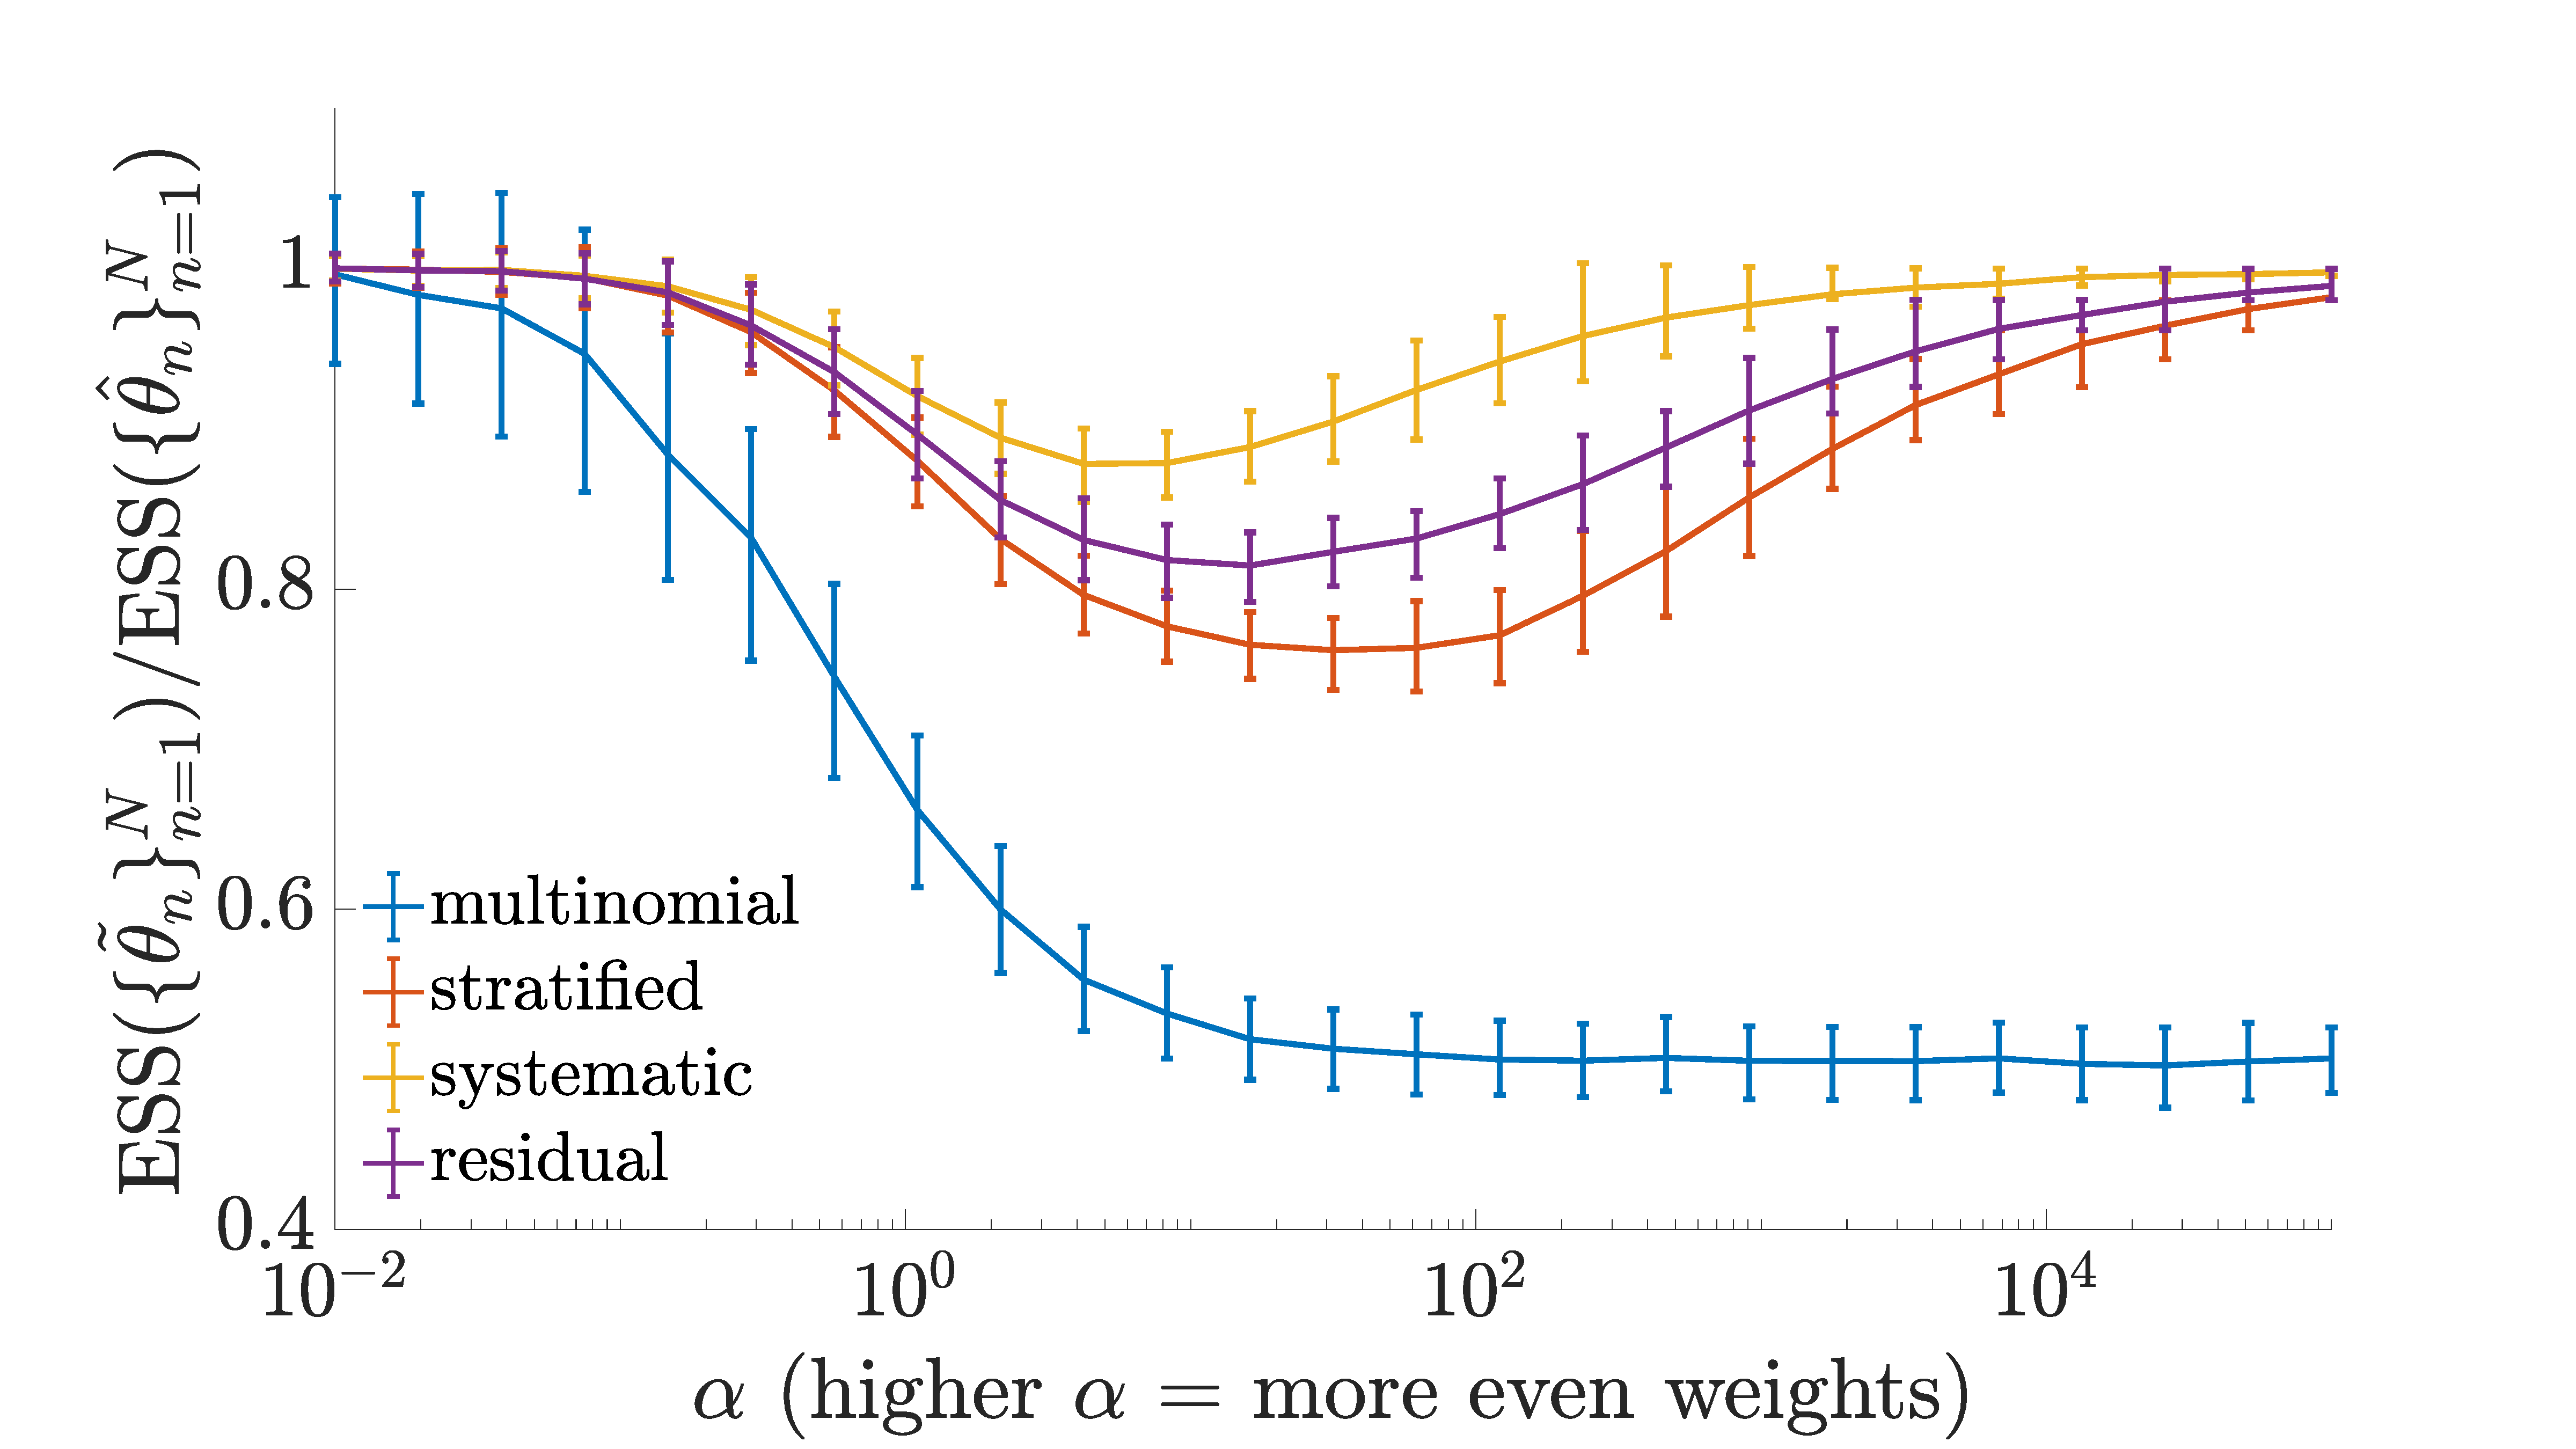
\includegraphics[width=\textwidth]{resampling100}
	\caption{Sample set size $N=100$}
	\end{subfigure}
	~
	\begin{subfigure}[t]{0.49\textwidth}
	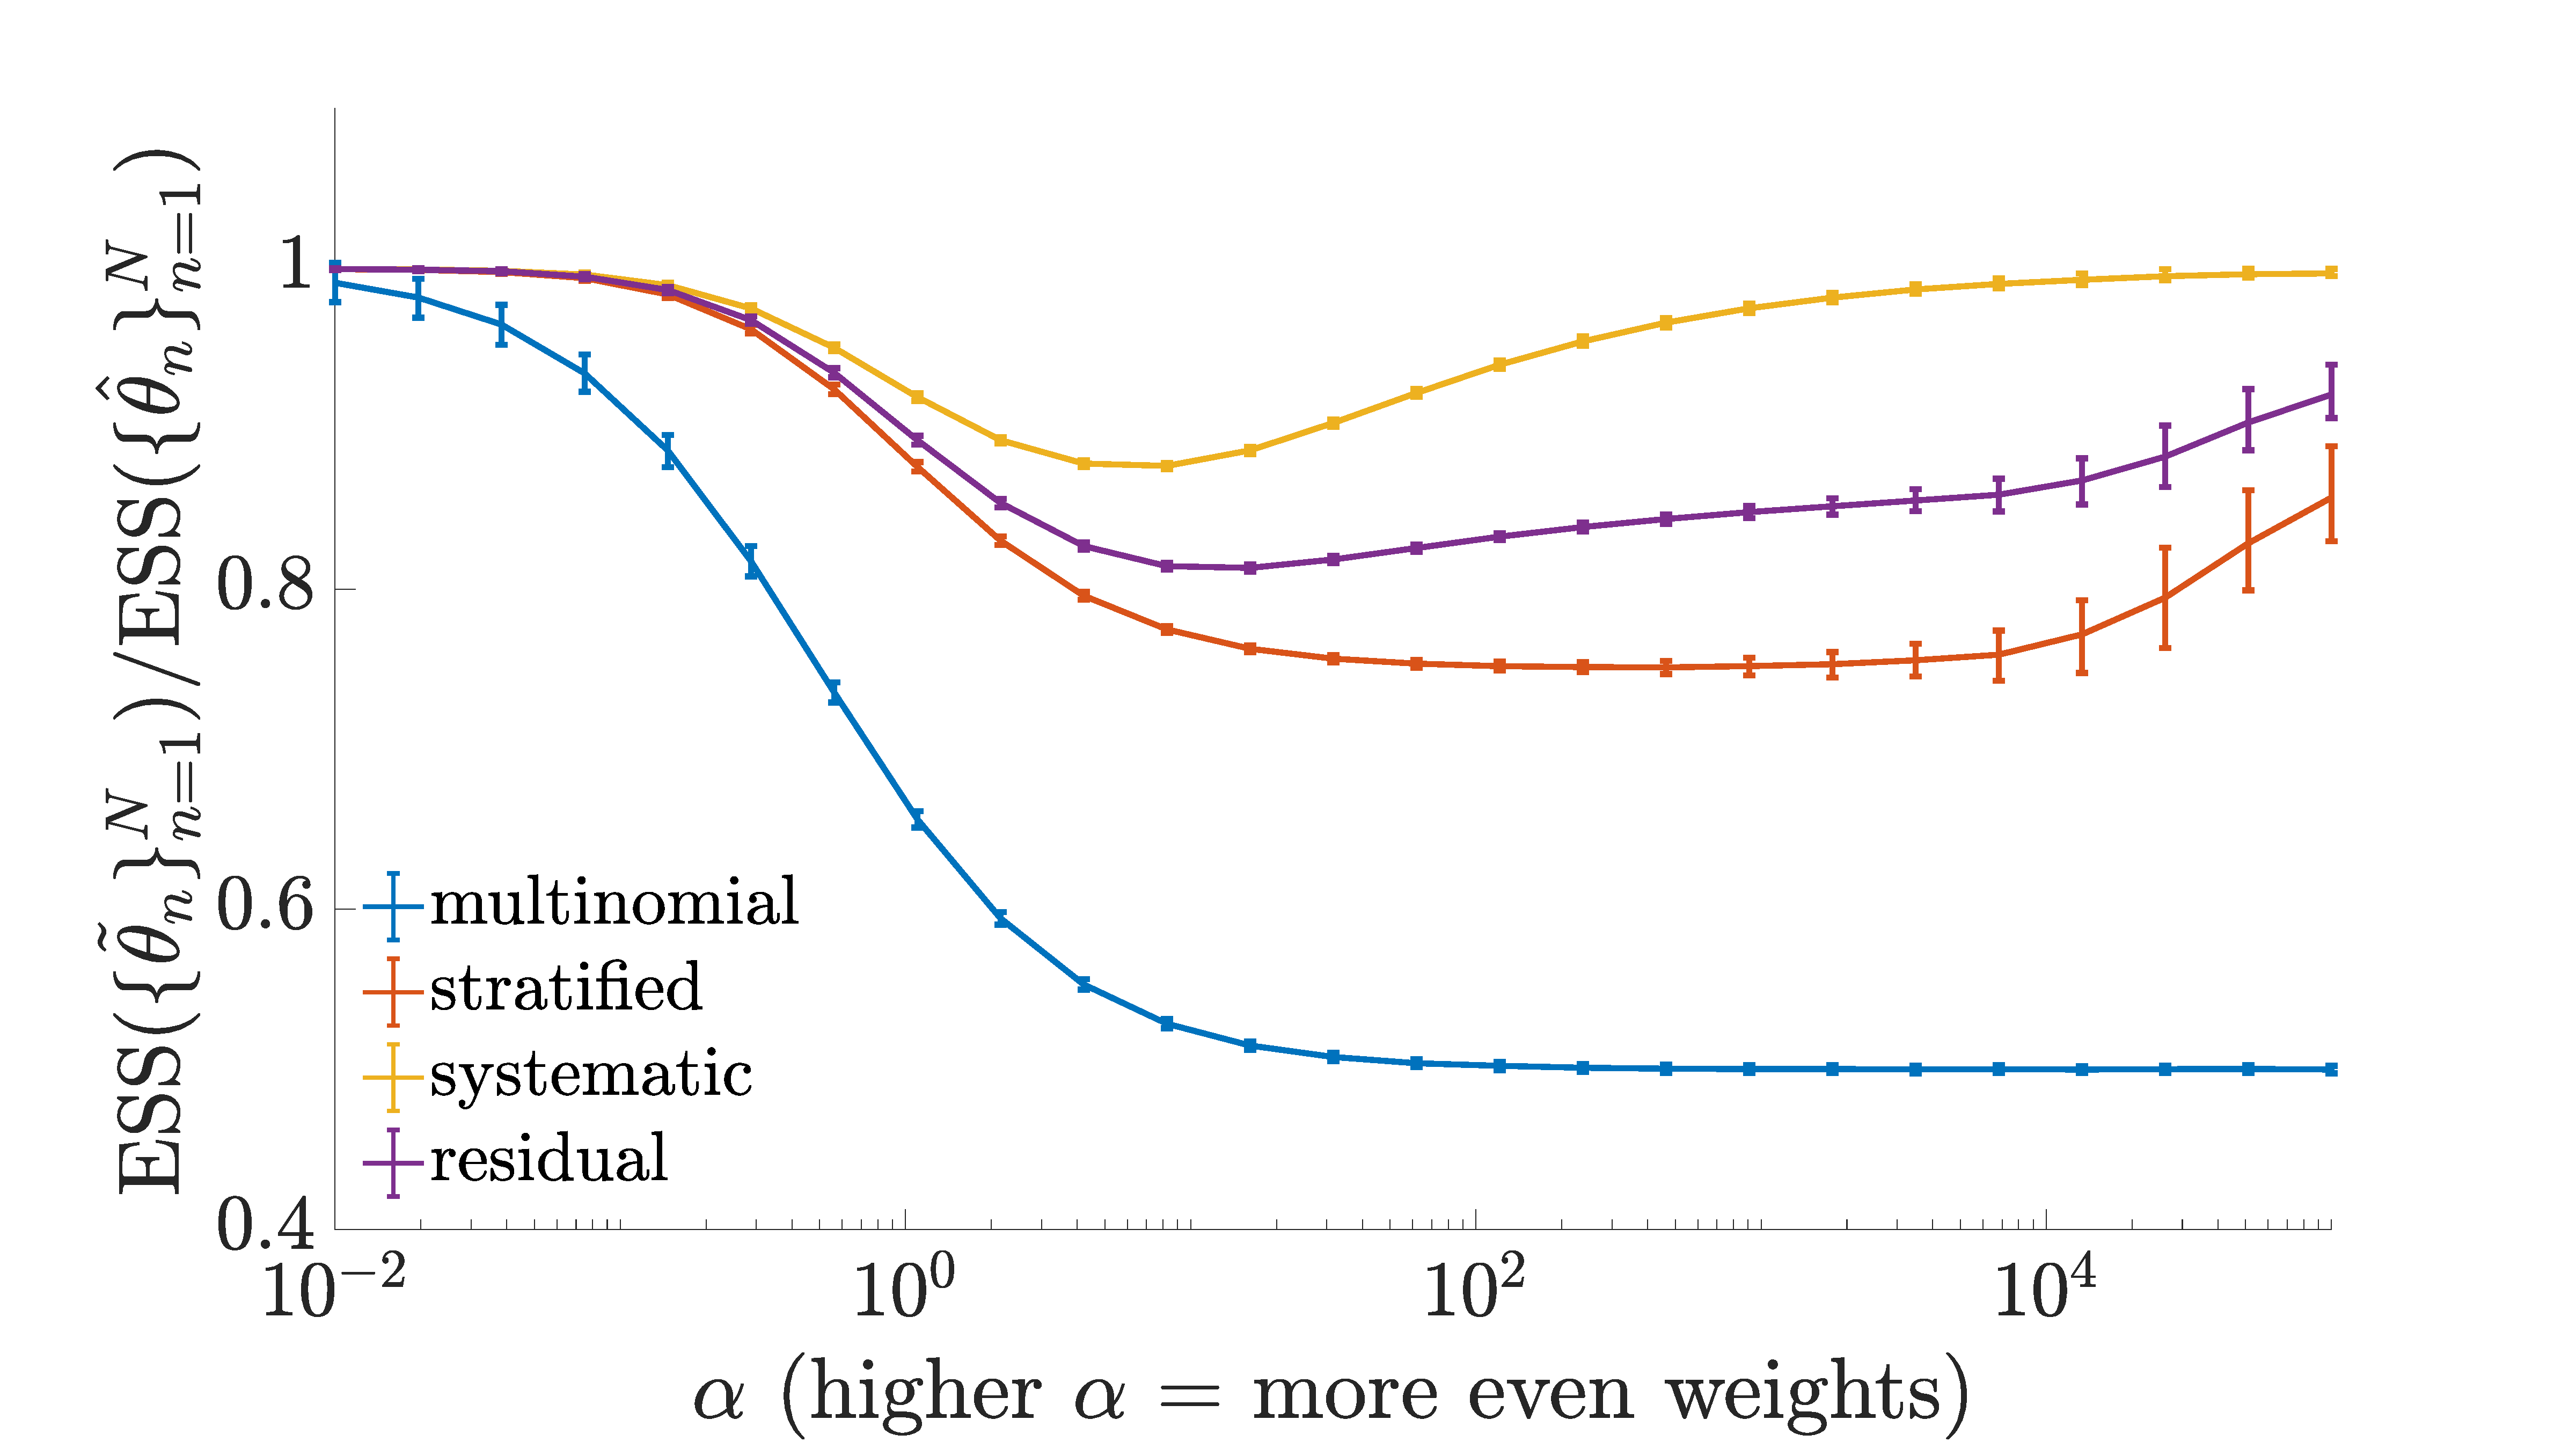
\includegraphics[width=\textwidth]{resampling10000}
	\caption{Sample set size $N=10000$}
	\end{subfigure}
	\caption{Demonstration of performance of different resampling schemes for
		two different sample set sizes and different levels of variance in the weights.
		Plots are generated by first sampling a set of $N$ weights from a symmetric
		Dirichlet distribution with parameter $\alpha$, 
		$\{\bar{w}_n\}_{n=1}^N \sim \textsc{Dirichlet}(\alpha)$, such that the
		higher $\alpha$ is, the more even the weights are on average.  The effective
		sample size (ESS) as defined in~\eqref{eq:inf:ess} is then calculated before an after the
		resampling is carried out (with identical samples collapsed to a single sample), and the ratio 
		reported.  Plots show the mean across $1000$ independent trials, with the
		error bars corresponding the to the interquartile range.
		\label{fig:inf:resample}}
\end{figure}

An empirical assessment of the methods is shown in Figure~\ref{fig:inf:resample}.  This shows
the relative effective sample size (ESS) before an after resampling as a function of the uniformity of
the weights.  To calculate the ESS after the resampling, we collapse the identical duplicated
particles down to a single sample with the combined weight of the other samples.  This is equivalent
to replacing $w_n$ with $k_n/N$ in the ESS calculation given in~\eqref{eq:inf:ess}.
Figure~\ref{fig:inf:resample} shows that systematic resampling is clearly preferable to the alternatives, at least
in the terms of the ESS after resampling for this particular problem, with this improvement consistent across the different
sample size sets.  Similar relatives performances are found if one instead uses the proportion of samples that
survive the resampling as a performance metric.
As expected, multinomial resampling is significantly worse than the other
methods, particularly when the weights are more even.  The results also suggest that residual
resampling outperforms stratified resampling, though this can come at the cost of being more
complicated to implement and potentially slower to run.  
%Note that the reason the ESS sometimes
%rises above $1$ for a particular trial is because it is an imperfect measure of the information 
%stored in the samples and so this simply happens by chance.